% Capítulo 9: seleção de atividades, palestras ordenadas pelo horário de término.
\documentclass[border=4pt]{standalone}
\usepackage[utf8]{inputenc}
\usepackage[T1]{fontenc}
% Estilo comum das figuras de vetores (capítulo 8).
\usepackage{tikz}
\usetikzlibrary{arrows.meta, positioning, calc, decorations.pathreplacing}
\definecolor{navy}{RGB}{23,45,80}
\definecolor{laranja}{RGB}{250,110,29}
\definecolor{cinzalogo}{RGB}{107,114,126}
\definecolor{azul}{RGB}{205,222,247}
\tikzset{
  casa/.style={draw=navy, line width=0.9pt, minimum width=8mm, minimum height=7mm,
               inner sep=0pt, font=\sffamily\small},
  pronta/.style={casa, fill=azul},
  parte/.style={casa, fill=laranja!12},
  marcada/.style={casa, fill=laranja!45, draw=laranja},
  fora/.style={casa, draw=cinzalogo!60, dashed, fill=white, text=cinzalogo!60},
  indice/.style={font=\sffamily\scriptsize, text=cinzalogo},
  explica/.style={font=\sffamily\small, text=navy, anchor=east},
  legenda/.style={font=\sffamily\scriptsize, text=cinzalogo},
  rotulo/.style={font=\sffamily\small\bfseries, text=navy},
  seta/.style={-{Stealth[length=2.2mm]}, navy, line width=0.9pt},
  chave/.style={decorate, decoration={brace, amplitude=4pt, mirror}, navy, line width=0.8pt},
}
% \vetor{nome}{x}{y}{valor/estilo, valor/estilo, ...}: casas lado a lado, chamadas nome0, nome1...
\newcommand{\vetor}[4]{%
  \foreach \valor/\estilo [count=\i from 0] in {#4} {
    \node[\estilo] (#1\i) at ($(#2, #3) + (\i*0.8, 0)$) {\valor};
  }
}

\tikzset{
  barra/.style={draw=cinzalogo, fill=cinzalogo!15, line width=0.6pt, rounded corners=1pt},
  escolhida/.style={draw=laranja, fill=laranja!45, line width=0.9pt, rounded corners=1pt},
  nome/.style={font=\sffamily\small, text=navy, anchor=east},
}
\begin{document}
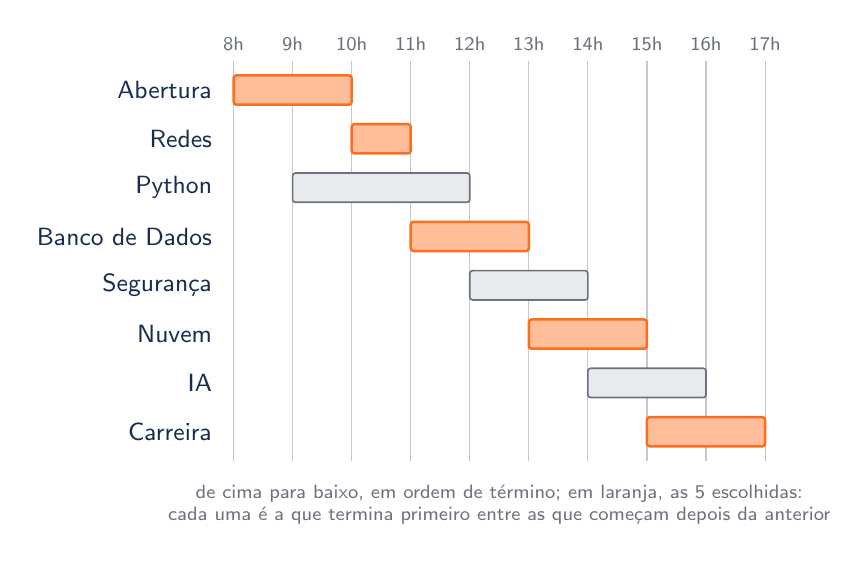
\begin{tikzpicture}[x=0.75cm, y=0.62cm]
  % eixo das horas (8h às 17h)
  \foreach \h in {8,...,17} {
    \draw[cinzalogo!40] (\h, 0.6) -- (\h, -7.6);
    \node[indice] at (\h, 0.95) {\h h};
  }
  \foreach \nome/\ini/\fim/\estilo [count=\k from 0] in
    {Abertura/8/10/escolhida, Redes/10/11/escolhida, Python/9/12/barra,
     Banco de Dados/11/13/escolhida, Segurança/12/14/barra, Nuvem/13/15/escolhida,
     IA/14/16/barra, Carreira/15/17/escolhida} {
    \draw[\estilo] (\ini, -\k - 0.3) rectangle (\fim, -\k + 0.3);
    \node[nome] at (7.8, -\k) {\nome};
  }
  \node[legenda, align=center] at (12.5, -8.5)
    {de cima para baixo, em ordem de término; em laranja, as 5 escolhidas:\\
     cada uma é a que termina primeiro entre as que começam depois da anterior};
\end{tikzpicture}
\end{document}
